\RequirePackage{silence}
\WarningFilter{hyperref}{Token not allowed}
\WarningFilter{microtype}{tracking amount}
\WarningFilter{chessfss}{\comment already}

% Transparency mode (no overlays)
\documentclass[xcolor={x11names,svgnames,dvipsnames},trans]{beamer}

\usepackage{pgfpages}
\usepackage{subfig}
\usepackage{tikz}
\usetikzlibrary{arrows,shapes,positioning,shadows,trees}

\usepackage[british]{babel}

%% Glossy pretty look for the presentation and transparency (w/o overlays and animations) versions!
\mode<beamer|trans>{
\useoutertheme[glossy]{wuerzburg}
\useinnertheme[shadow,outline]{chamfered}
\usecolortheme{shark}
}
\setbeamertemplate{navigation symbols}{}
\setbeamertemplate{frametitle continuation}[from second][(cont'd)]
\usefonttheme[stillsansseriftext,stillsansserifsmall]{serif}

%% Save up on ink for the 4-up handouts
\mode<handout>{
\useoutertheme{wuerzburg}
\useinnertheme[outline]{chamfered}
%\pgfpagesuselayout{4 on 1}[a4paper, landscape, border shrink=10mm]
\pgfpagesuselayout{2 on 1}[a4paper, border shrink=10mm]
\pgfpageslogicalpageoptions{1}{border code=\pgfstroke}
\pgfpageslogicalpageoptions{2}{border code=\pgfstroke}
%\pgfpageslogicalpageoptions{3}{border code=\pgfstroke}
%\pgfpageslogicalpageoptions{4}{border code=\pgfstroke}
\setbeamercolor{structure}{fg=black}
\setbeamercolor{alerted text}{fg=black}
}

\mode<presentation>{\AtBeginSection[]{%
\begin{frame}
\frametitle{Contents}
\tableofcontents[currentsection]
\end{frame}}}

\usepackage[T1,safe]{tipa}
\usepackage{microtype}
\usepackage[utf8]{inputenc}
\usepackage[T1]{fontenc}
\usepackage{libertine}
\usepackage[scaled=.77]{beramono}
\SetTracking{encoding=*}{-39}

\usepackage{relsize,tabularx}
\usepackage{hologo,textcomp}
\usepackage{comment}
\usepackage[skaknew]{chessboard,skak}
\usepackage{multicol,booktabs}
\usepackage{listings}
\lstset{upquote,keepspaces=true,columns=spaceflexible,
basicstyle=\ttfamily\scriptsize,%
breaklines=true,breakindent=0pt,xleftmargin=0pt, xrightmargin=6pt,%
language=[LaTeX]TeX, texcsstyle=*\bfseries\color{Maroon}, commentstyle=\sffamily\itshape\smaller\color{SeaGreen4},
emphstyle=\bfseries\color{RoyalBlue3},escapechar={:},
emphstyle={[2]{\bfseries\color{Sienna2}}},
postbreak=\mbox{{\smaller\color{gray}$\hookrightarrow$}}
}

\mode<handout>{
   \lstset{
   texcsstyle=*\bfseries, commentstyle=\sffamily\itshape\smaller,
   emphstyle=\bfseries,escapechar={:},
   emphstyle={[2]{\bfseries}},
   emphstyle={[3]{\bfseries}},
   postbreak=\mbox{{\smaller$\hookrightarrow$}}
   }
}

\makeatletter
\lst@CCPutMacro\lst@ProcessOther {"2D}{\lst@ttfamily{-{}}{-{}}}
\@empty\z@\@empty
\makeatother


\usepackage{pgfgantt}
\usetikzlibrary{backgrounds}

\usepackage{multicol,multirow}
\usepackage[version=3]{mhchem}
\usepackage{chemfig}
\usepackage{expex,qtree}
\usepackage{texshade}
\usepackage[detect-all]{siunitx}
\usepackage[siunitx]{circuitikz}
\usepackage{smartdiagram}
\usepackage{bytefield}
% \usepackage{pstricks,pst-barcode}
% \usepackage{auto-pst-pdf}
\usepackage{pgfplots}
\pgfplotsset{compat=1.12}
\usepackage{cwpuzzle}
\usepackage{gchords,guitar}
\usepackage{spreadtab}
\usepackage{ccicons}
\usepackage{marvosym}
\usepackage{upgreek}
\usepackage{adforn}
% \ifpdf
\pdfmapfile{+webo.map}
% \fi
\newcommand{\wb}[1]{{\usefont{U}{webo}{xl}{n}#1}}
\usepackage{bookmark}

\setlength\fboxsep{0pt}

\author[Omar Gutiérrez]{\texorpdfstring{Omar Gutiérrez}{Omar Gutiérrez}}
\title{Review of TransG}
\subtitle{\texorpdfstring{\textsc{A Generative Model for Knowledge Graph Embedding}\\%
\hrulefill\ \adforn{57}\thickspace\thickspace\adforn{29}\ \hrulefill}{}}
\date[\ccbyncsa]{\ccbyncsa}

%\titlegraphic{\includegraphics[width=.3\textwidth]{TFZsuperellipse-crop}\\\tiny Illustration by Duane Bibby}

\hypersetup{%
pdfauthor={Omar Gutiérrez},
pdfkeywords={TransG}
}

\begin{document}
\begin{frame}[plain]
\maketitle
\end{frame}

\begin{frame} \frametitle{Contents}
    \tableofcontents
\end{frame}

%-=-=-=-=-=-=-=-=-=-=-=-=-=-=-=-=-=-=-=-=-=-=-=-=
%	SECTION: Introduction
%-=-=-=-=-=-=-=-=-=-=-=-=-=-=-=-=-=-=-=-=-=-=-=-=

\section{Introduction}

%-=-=-=-=-=-=-=-=-=-=-=-=-=-=-=-=-=-=-=-=-=-=-=-=
%	FRAME: Introduction
%-=-=-=-=-=-=-=-=-=-=-=-=-=-=-=-=-=-=-=-=-=-=-=-=

\subsection{Overview}
\begin{frame}{Overview}
    \begin{itemize}
        \item Traditional knowledge bases are symbolic and logic.
        \item Thus, numerical machine learning methods are not compatible with these databases.
        \item \textbf{Solution}: Knowledge Graph Embedding (KGE).
        \item The idea of KGE is convert entities and relations into continuous vector spaces.
        \item Several solutions have been proposed: TransE, Latent Factor Model, RESCAL, etc.
        \item \textbf{TransG} was proposed in 2015.
        \item Its main contribution is introduce and solve the issue of \textbf{multiple relation semantics}.
    \end{itemize}
\end{frame}

\subsection{Translation-Based Embedding Methods}
\begin{frame}{Translation-Based Embedding Methods}

    \begin{itemize}
        \item A family of embedding models is known as translation-based.
        \item \textbf{TransE} is the most significant work.
    \end{itemize}

    \begin{center}
        \begin{minipage}{.8\textwidth}\rmfamily
            \begin{itemize}
                \item Translation principle: $$ h + r \approx t$$
                \item Score function: $$ f_r(h, t) = \| h_r + r - t_r\|_2^2 $$
            \end{itemize}
        \end{minipage}
    \end{center}

    \begin{itemize}
        \item Several modifications have been proposed:
        \item TransH, TransR, CTransR, TransM, and KG2E
    \end{itemize}

\end{frame}

\subsection{Other Embedding Methods}
\begin{frame}{Other Embedding Methods}
    \begin{itemize}
        \item \textbf{Structured and unstructured embedding}
        \item \textbf{Neural Network based Embedding}: Single Layer Model, Neural Tensor Network
        \item \textbf{Factor models and matrix factorization}: Latent Factor Model, RESCAL
    \end{itemize}
\end{frame}

\subsection{Multiple Relation Semantics}
\begin{frame}{Multiple Relation Semantics}
    \begin{itemize}
        \item A relation may have \textbf{multiple meanings}, depending on the associated entity pairs:
            \begin{itemize}
                \item Composition: \texttt{<Table, HasPart, Leg>}
                \item Location: \texttt{<Atlantics, HasPart, NewYorkBay>}
            \end{itemize}
        \item Why?
            \begin{itemize}
                \item \textbf{Simplification:} Abstracting multiple similar relations into one specific is a common trick
                \item \textbf{Nature of knowledge:} Ambiguous information
            \end{itemize}
        \item The ambiguity of knowledge means a semantic mixture
    \end{itemize}
\end{frame}

\begin{frame}{Multiple Relation Semantics II}

    {\centering
    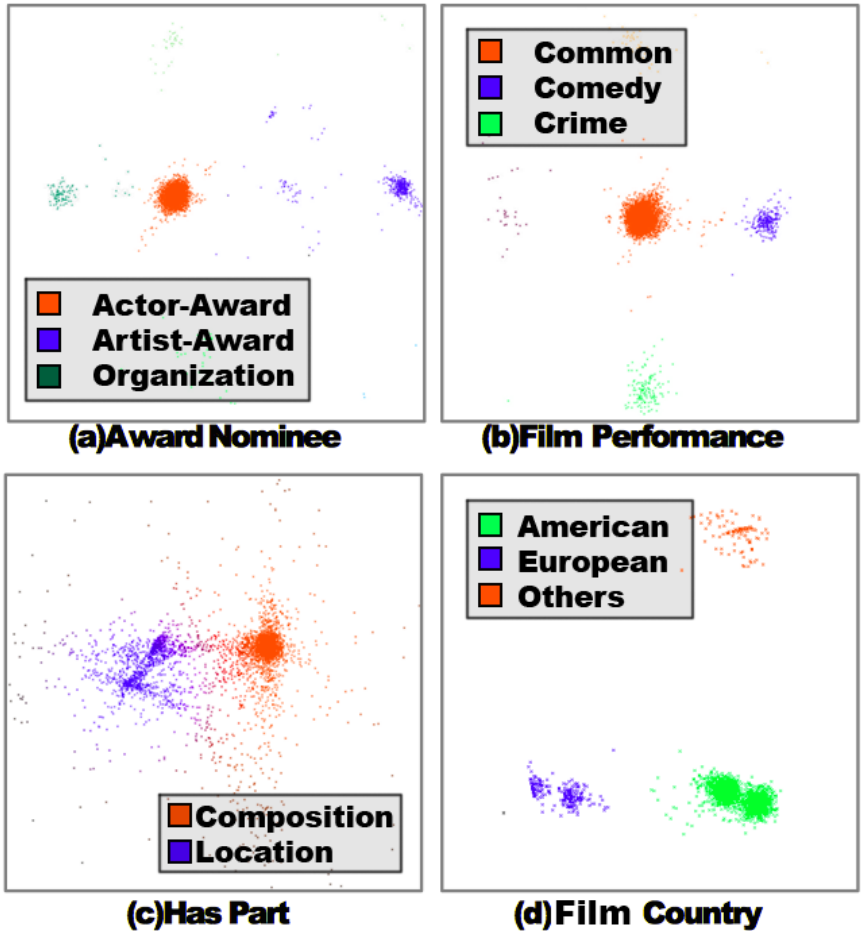
\includegraphics[width=0.45\textwidth]{images/pca.png}\par
    }

    \begin{itemize}
        \item This PCA dimension reduction visualization shows TransE embedding vectors
        \item With TransE there is only one cluster whose center is the vector $r$
    \end{itemize}
\end{frame}

\begin{frame}{Multiple Relation Semantics III}

    {\centering
    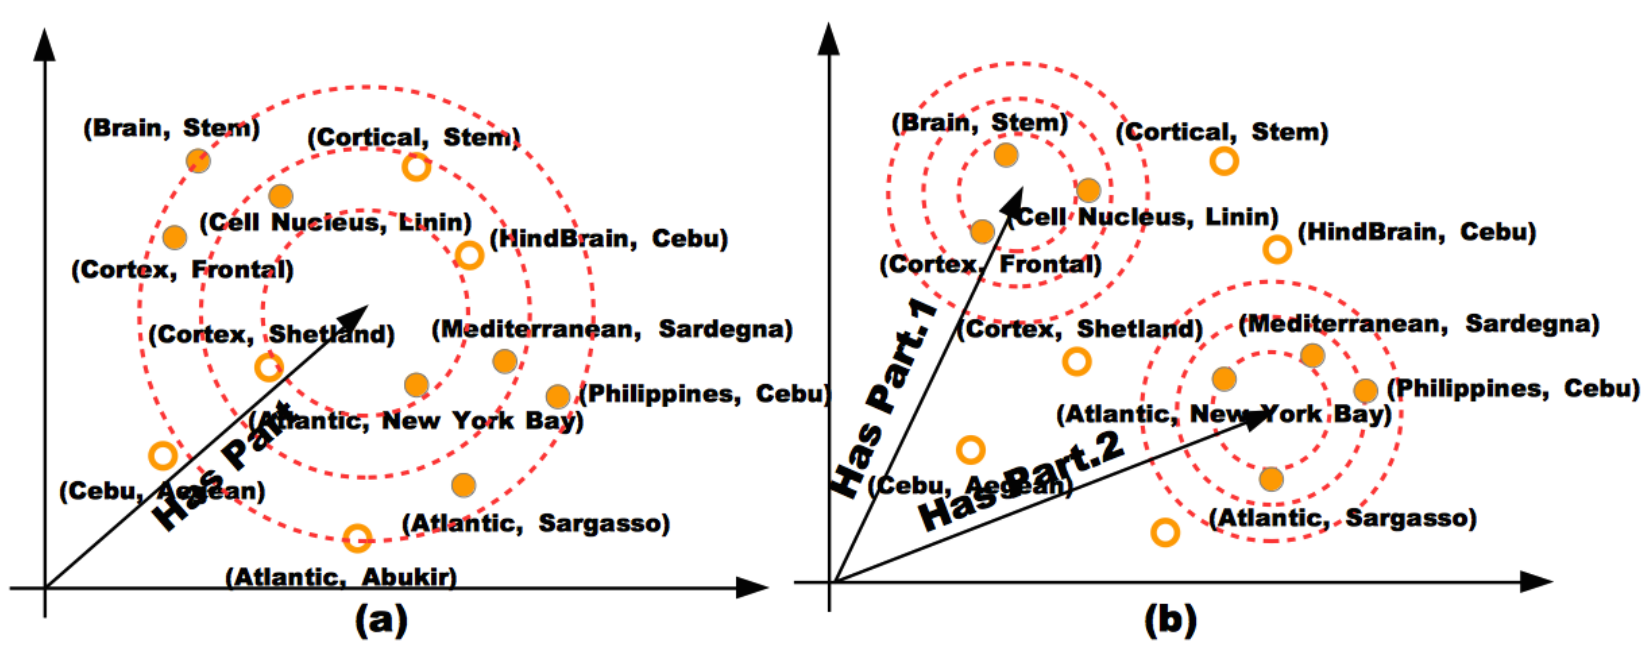
\includegraphics[width=0.90\textwidth]{images/clustering.png}\par
    }

\end{frame}

\section{Methods}
\subsection{Bayesian nonparametric models}
\begin{frame}{Bayesian nonparametric models}

    \begin{center}
        \begin{minipage}{.9\textwidth}\rmfamily
            TransG is a \textbf{Bayesian nonparametric infinite mixture model}
        \end{minipage}
    \end{center}

    \begin{figure}[H]
        \centering
        
\tikzset{
  basic/.style  = {draw, text width=2cm, align=center, drop shadow, font=\sffamily\footnotesize, rectangle, fill=gray!30},
  root/.style   = {basic, rounded corners=2pt, thin},
  level 2/.style = {basic, rounded corners=6pt, thin, text width=6em},
  level 3/.style = {basic, rounded corners=2pt, thin, text width=5em},
  level 4/.style = {basic, rounded corners=2pt, thin, text width=6em, font=\tiny}
}

\begin{tikzpicture}[
  level 1/.style={sibling distance=40mm},
  edge from parent/.style={->,draw},
  edge from node/.style={->,draw, black},
  >=latex]

% root of the the initial tree, level 1
\node[root] {\textbf{Bayesian models}}
% The first level, as children of the initial tree
  child {node[level 2] (c1) {Parametric}}
  child {node[level 2] (c2) {\textbf{Nonparametric}}
    child {node[level 3] (c21) {\textbf{Mixture}}
        child {node[level 4] (c211) {\textbf{Chinese Restaurant\\ Process}}}
    }
    child {node[level 3] (c22) {Latent factor}
        child {node[level 4] (c221) {Indian Buffet\\ Process}}
    }
  };

\node (comment) [above left = of c1] {Finite};
    \draw [->, thick] (comment) to [in = 110] (c1);

\node (comment2) [above right = of c2] {Infinite};
    \draw [->, thick] (comment2) to [in = 110] (c2);


% The second level, relatively positioned nodes
%\begin{scope}[every node/.style={level 3}]
%\node [below of = c1, xshift=15pt] (c11) {Setting shape};
%\node [below of = c11] (c12) {Choosing color};
%\node [below of = c12] (c13) {Adding shading};

%\node [below of = c2, xshift=15pt] (c21) {Using a Matrix};
%\node [below of = c21] (c22) {Relatively};
%\end{scope}

% lines from each level 1 node to every one of its "children"
%\foreach \value in {1,2,3}
%  \draw[->] (c1.195) |- (c1\value.west);

%\foreach \value in {1,...,4}
%  \draw[->] (c2.195) |- (c2\value.west);

\end{tikzpicture}

        %\caption{Bayesian models}
    \end{figure}

\end{frame}

\begin{frame}{Bayesian parametric vs nonparametric models}
    \begin{itemize}
        \item Traditional approach (finite)
           \begin{itemize}
               \item The number of parameters $\theta$ (e.g. clusters) is prespecified
               \item We have a prior distribution over parameters $P(\theta)$
               \item For example, in the Gaussian mixture model, each cluster will be modelled
                   using a parametric model (e. g. Gaussian)
           \end{itemize}
        \item Bayesian nonparametric models
           \begin{itemize}
               \item We assume that there is an \textbf{infinite} number of latent clusters
               \item A finite number of clusters is \textit{inferred} from data
               \item The number of clusters grow as new data points are observed
           \end{itemize}
    \end{itemize}

\end{frame}

\begin{frame}{Chinese Restaurant Process}

    {\centering
    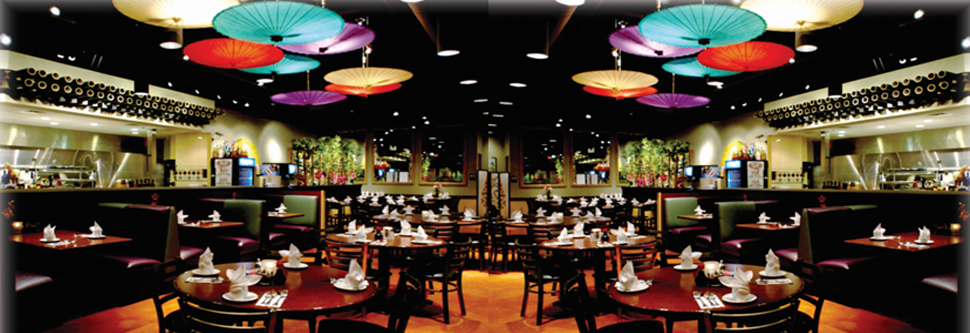
\includegraphics[width=0.75\textwidth]{images/crp.png}\par
    }

    \pause

    \begin{itemize}
        \item Imagine a restaurant with an infinite number of tables,
        \item and a sequence of customers entering the restaurant and sitting down.
        \item The first customer enters and sits at the first table
        \item The second customer enters and sits...
            \begin{itemize}
                \item at the first table with probability $\frac{1}{1 + \alpha}$
                \item at the second table with probability $\frac{\alpha}{1 + \alpha}$
            \end{itemize}
        \item We realize that CRP is a form of clustering: $K$ groups and each group with size $N_k$
    \end{itemize}
\end{frame}

\begin{frame}{Generative Process}

    {\centering
    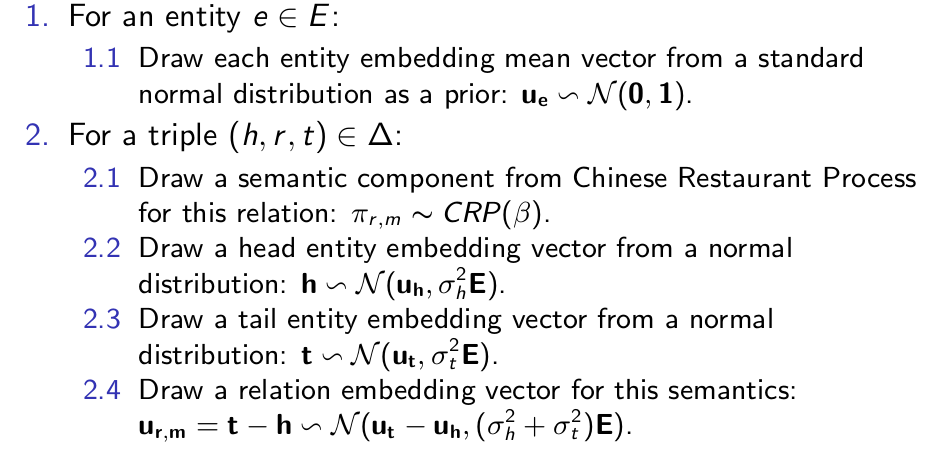
\includegraphics[width=0.75\textwidth]{images/algorithm.png}\par
    }

    \begin{center}
        \begin{minipage}{.8\textwidth}\rmfamily
            \begin{itemize}
                % \item Score function: $$ f_r(h, t) = \| h_r + r - t_r\|_2^2 $$
                \item Translation principle from $ h + r \approx t$ becomes
                   {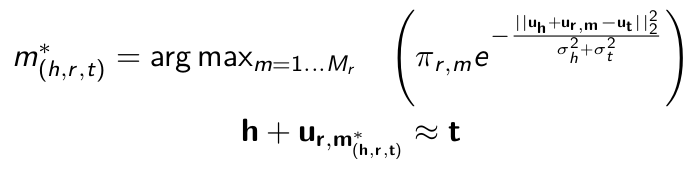
\includegraphics[width=0.75\textwidth]{images/geometrical.png}\par
                   }
                \item Notice that $r$ is has a selective translation
            \end{itemize}
        \end{minipage}
    \end{center}

\end{frame}

\section{Experiments}

\begin{frame}{Experiments}

    \begin{itemize}
        \item The experiments were carried out in benckmark datasets subsets of Freebase and Wordnet
        \begin{itemize}
            \item WN18, WN11, FB13, FB15K
            \item Raw setting:
            \item Filter setting: corrupted triples are filtered from test dataset.
        \end{itemize}
    \end{itemize}

\end{frame}

\subsection{Link Prediction}
\begin{frame}{Link Prediction}


    \begin{figure}[H]
        {\centering
        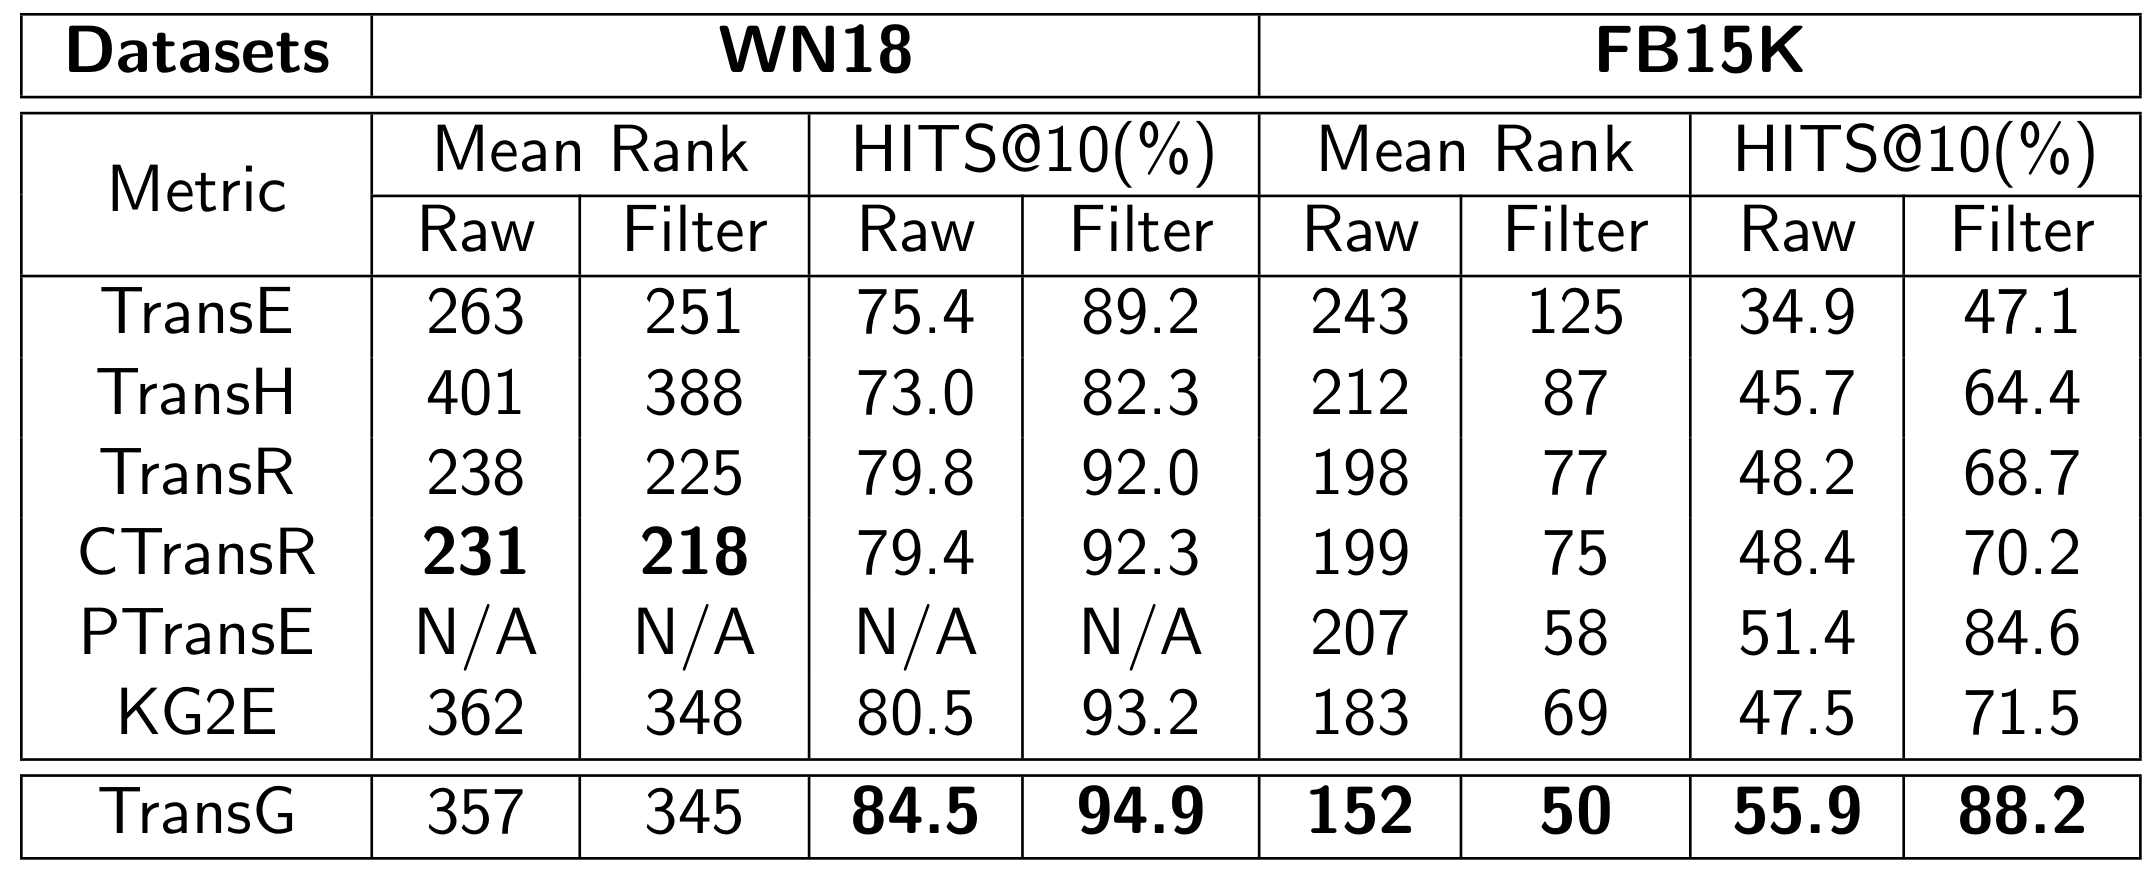
\includegraphics[width=0.75\textwidth]{images/link.png}\par
        }
    \caption{Evaluation results on link prediction}
    \end{figure}

    \begin{itemize}
        \item Lower \textbf{Mean Rank} and higher \textbf{HITS@10} mean better performance
    \end{itemize}

\end{frame}

\subsection{Triple Classification}
\begin{frame}{Triple Classification}

    \begin{figure}[H]
        {\centering
        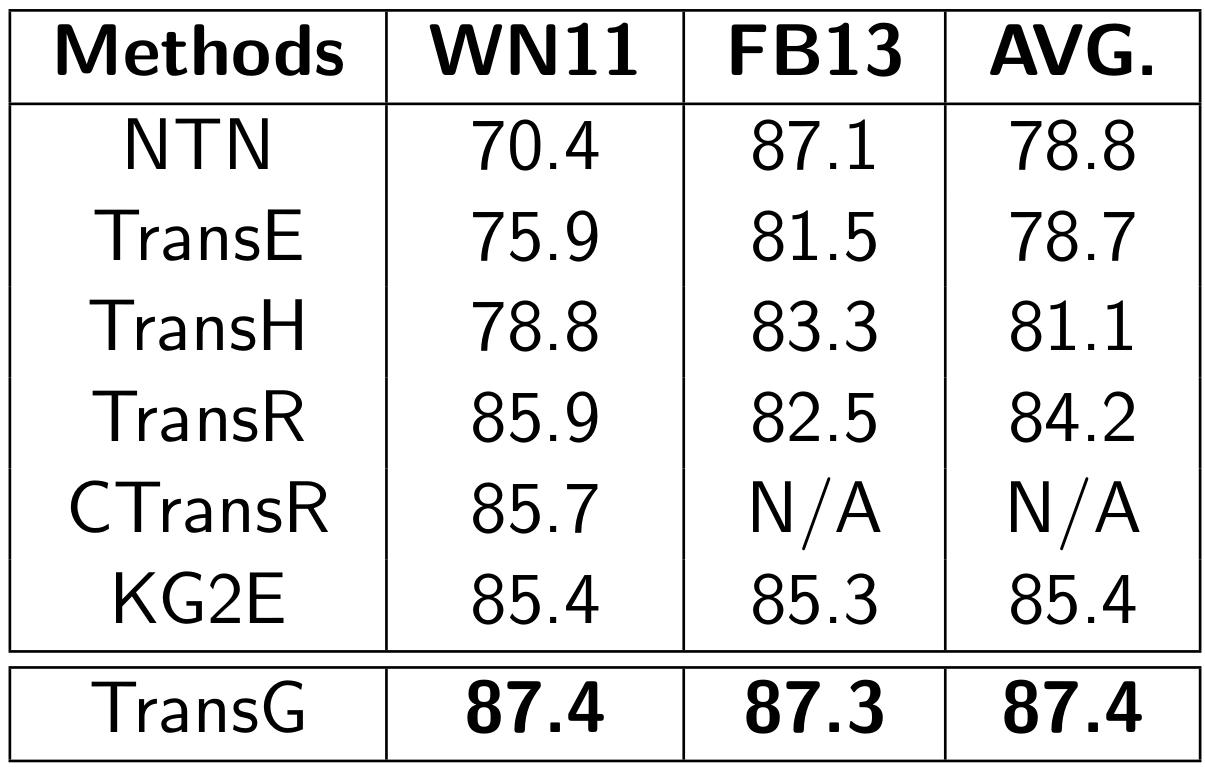
\includegraphics[width=0.55\textwidth]{images/triple.png}\par
        }
        \caption{Triple classification accuracy}
    \end{figure}

\end{frame}

\subsection{Semantic Component Analysis}

\section{Conclusions}
\begin{frame}{Conclusions}

    \begin{itemize}
        \item A solution for a new issue, commonly seen in knowledge graph, multiple relation semantics was presented with TransG
        \item Authors claim \textbf{substantial improvements} against the state-of-the-art baselines
            \begin{itemize}
                \item Still, TransE has 234 references and TransG has 1 reference
                \item O(TransG)  = (M x O(TransE)), TransE is one of the fastest methods for
            \end{itemize}
        \item We still have many letters in the alphabet to write more versions of Translation-Based methods \texttt{;)}
            \begin{itemize}
                \item For example, use another BNP to model the issue presented here.
            \end{itemize}
    \end{itemize}

\end{frame}

\end{document}
